\documentclass[12pt]{report}
\usepackage[utf8]{inputenc}
\usepackage{graphicx}
\usepackage{hyperref}

\title {
	
\includegraphics[width = .2\linewidth]{University-of-Lugano.png} \break \break
	{\bf\Huge Design Thinking}
	\\\large Human-Computer Interaction
	\\\small Academic Year 2017/2018 \break
	\\\large \textbf{Group 7}}
	\author{
	\\\large Alessandra Vicini \\ Edoardo Lunardi \\ Ozren Dabić \\ Pasquale Polverino \\ Paganoni Marco}
\date{March 19, 2018}
\begin{document}
	\pagestyle{empty}
	\maketitle

	\section*{\huge The Average User}
	By processing the data gathered during our contextual inquiry and analysis, we have since developed two polarising user personas:
	\begin{enumerate}
		\item {\large Maddalena Dellucci}\\
			\begin{itemize}
				\item Gender: Female
				\item Age: 12
				\item School: Istituto Elevetico Secondary School, First Year
				\item Sports/Hobbies:  Loves dancing and playing the violin.
				\item Description: She lives outside the centre, in a residential zone of Lugano. She rarely goes out with her friends and is usually not so comfortable in spending  time with children she is not familiar with. She is very shy and reserved, and she doesn't like take part in competitions. She performs exceptionally well in school but rarely participates during class sessions.
			\end{itemize}
		\item {\large Gerardino Trevisano}\\
				\begin{itemize}
					\item Gender: Male
					\item Age: 13
					\item School: Istituto Elevetico Secondary School, Second Year
					\item Sports/Hobbies: Plays soccer and basketball, loves all kinds of teams sports and competitions.
					\item Description: He lives in the centre of Lugano. He often goes out with his friends and loves spending his free time outside. He is outgoing, confident of his skills, and he has no fear of showing results. He frequents all manner of school activities and he enjoys being in the spotlight.
				\end{itemize}
	\end{enumerate}
	\newpage
	We chose two personas instead of one to represent the two majorities of our potential userbase. The first is a persona that represents children who generally have a harder time finding friends and who will use the app to create new friendships, in hopes of overcoming the fear of socialising with others. The second persona is a complete opposite of the first one. However it's important to note here that our "target population" is represented better by the first persona. The presence of the second persona should not be disregarded, as they too can benefit greatly from our application. However they represent a much broader audience, and satisfying their needs and demands comes after satisfying the needs of the first group.

	\section*{\huge Sketching and Ideation}
	Our next step was visualising our application in terms of ecological, emotional and interactive perspective. The visualisation process started out as a regular scribble and brainstorm session. Our first step was to discuss the gathered data, after which we began thinking of how all our observations and user requirements could fit into the app. We began visualising the app in use in the everyday environment, as well as the emotional impact it has on an individual. Furthermore, we constructed some design mockups. The first one we made was a "general application outline" in which we dissected core design features and minimal required technology to make some of those features achievable. We believe that pointing these out will not only allow us to build a better picture of what is needed in our application, but also what we could implement in the future to make the application more functional, more precise and more fun to use. The second one was a more direct sketch of the app in use with a generic prototype interface, demonstrating the functionality and flow of the UI. A key aspect was to both highlight the structure of the application as well as how this structure works with user interaction. We started with ideas like profiles and event search, gradually moving on to event creation, in app calendars, bookmarks, reminders, push notifications etc. Considering that a majority of our clients use smartphones and are familiar with how they work, we tried to base the design of our app around common design choices found in other apps, all the while keeping in mind that the use of our app has to be as simple as possible, reduced to actions like tap, swipe, and restricting writing to messages and search only.

	\section*{\huge Workspace and Materials}
	We would gather in the open space or in one of the smaller empty classrooms. During brainstorming, one person would draw, while the rest of the team discusses current data and information that we are in possession of in form of WAAD, all the while pointing out the context in which some of the concepts could fit into the app. All the drawings were done either on whiteboard or on paper.

	\section*{\huge Sketches}
	These are the sketches we produced:\\
	The first one is that of a general application outline.\\\\
	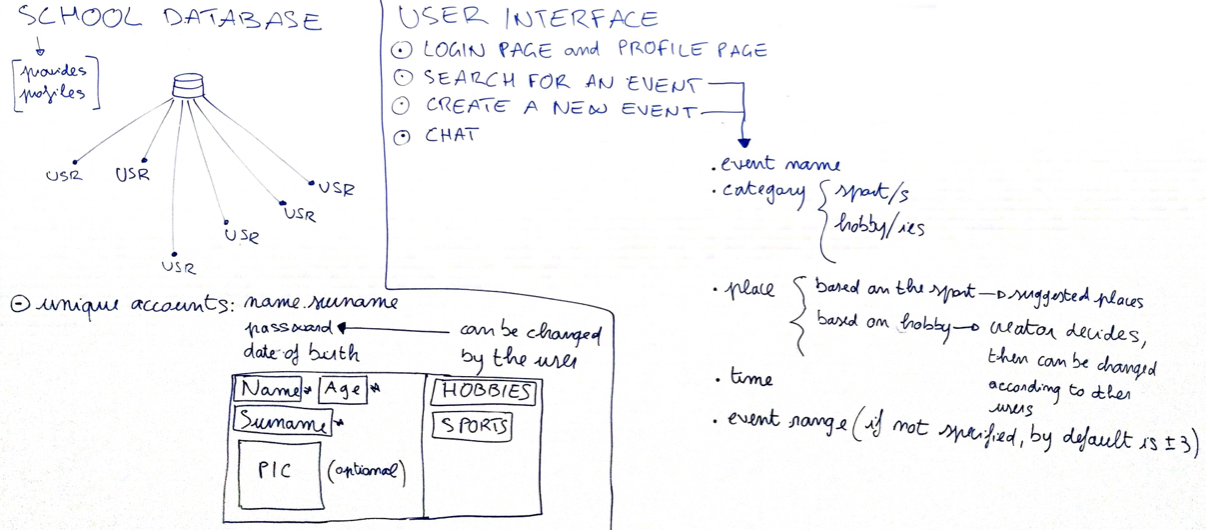
\includegraphics[width=\linewidth]{FirstDesign.jpg}\break
	\newpage

	Then we made a sketch of the interactive aspect of our app, showing some brief concepts of how it could be used:\\\\
	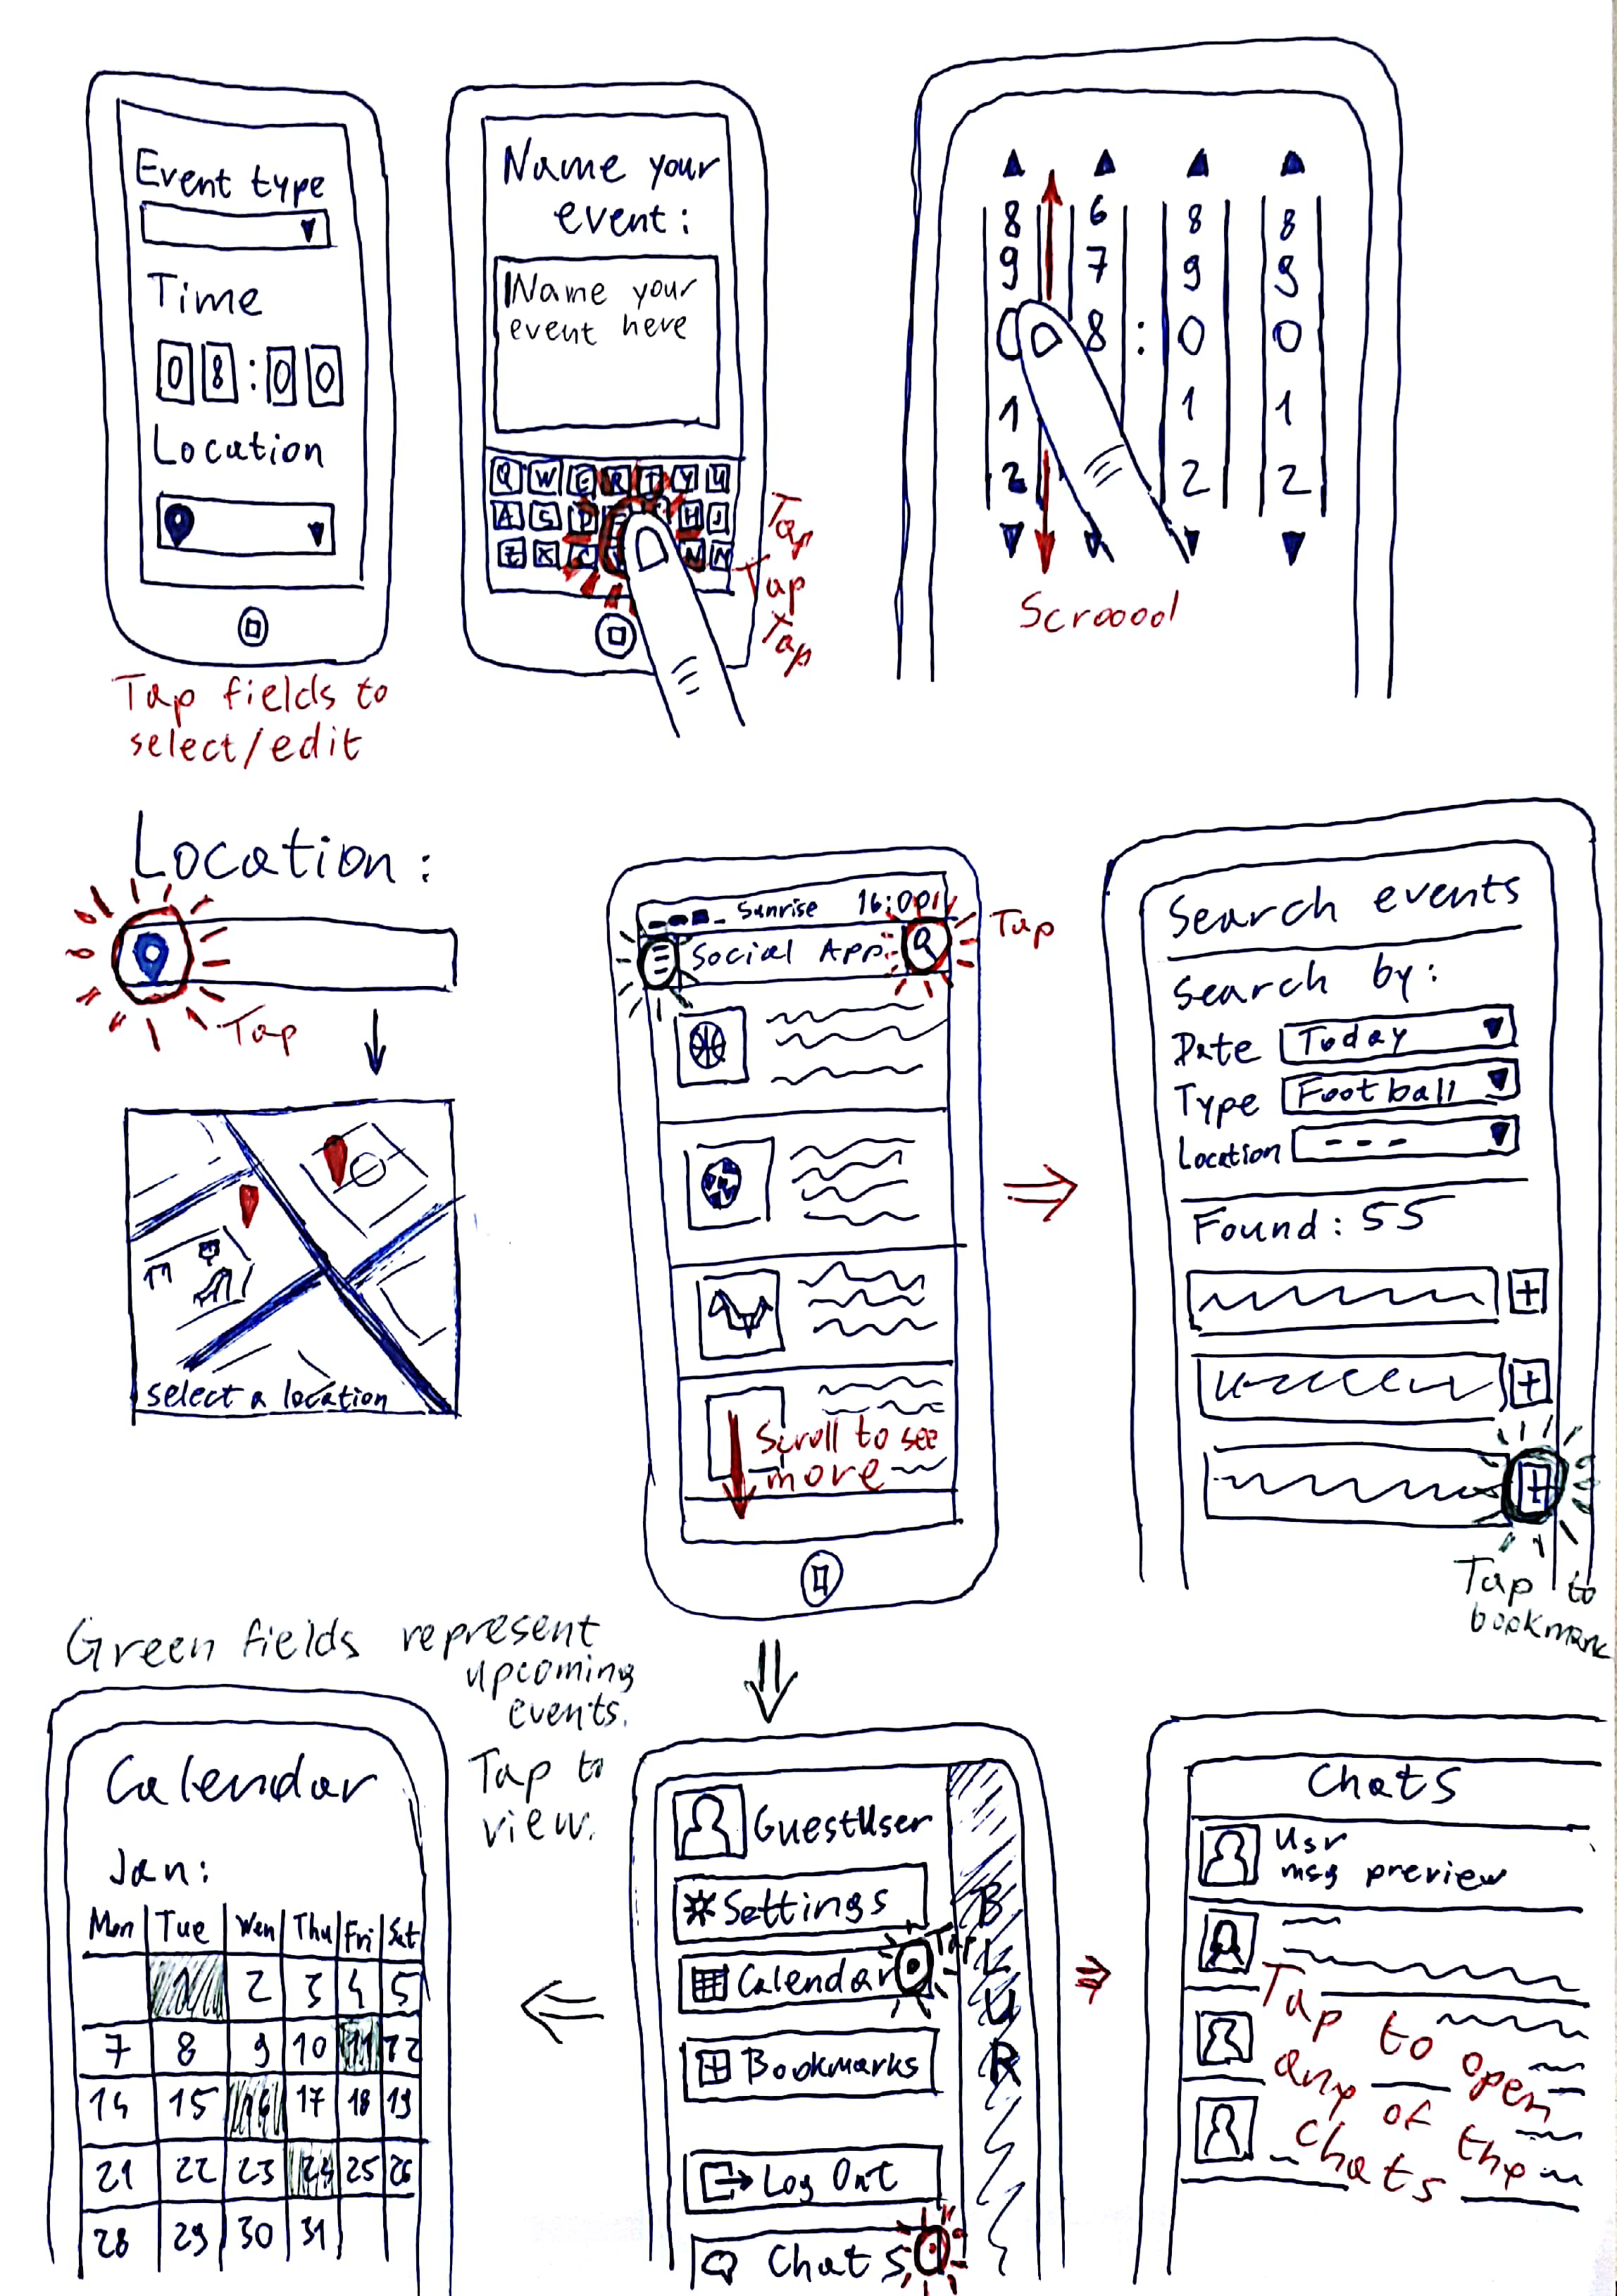
\includegraphics[scale=0.15]{Interaction.jpg}\break
	\newpage

	Then for the emotional aspect:\\\\
	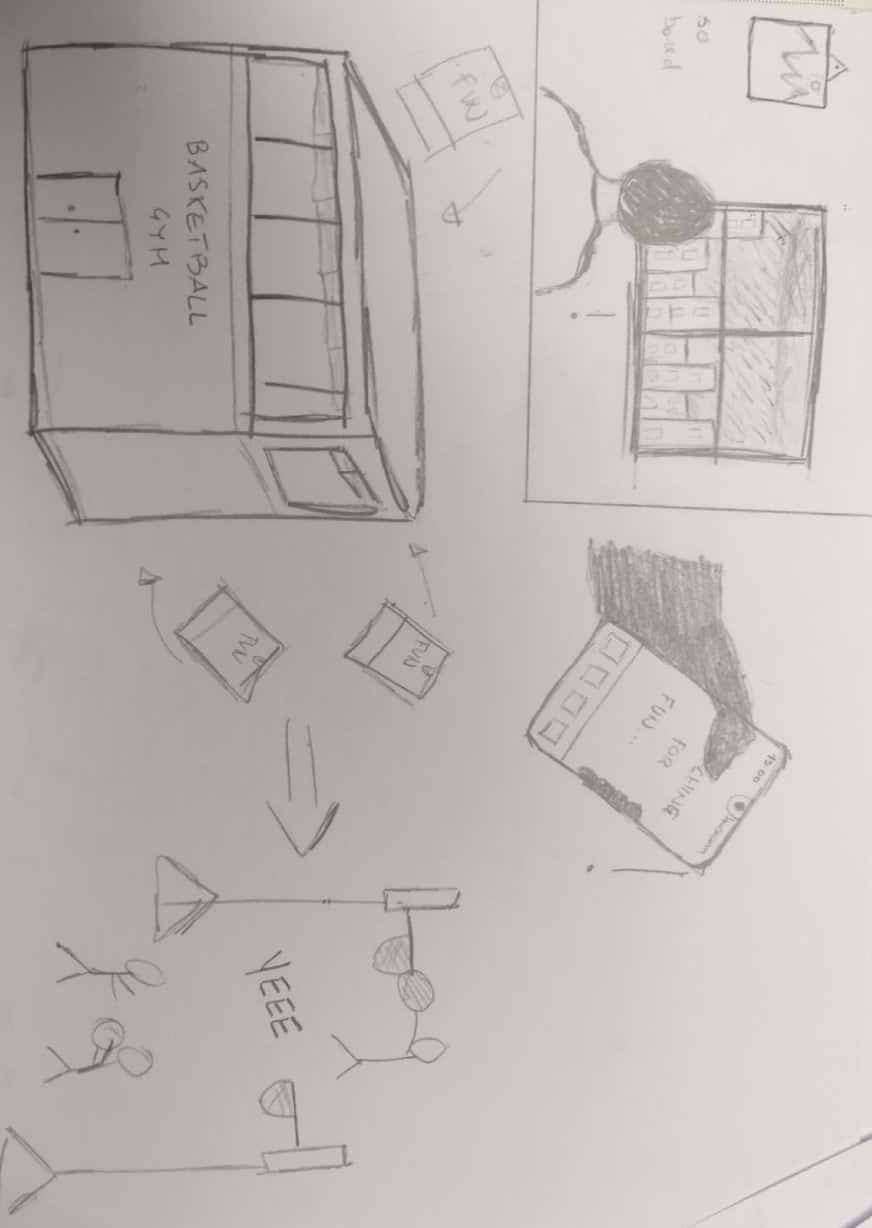
\includegraphics[scale=0.37]{Emotional.jpg}\break
	\newpage

	And lastly, for the ecological aspect, showcasing the the emotional impact that the app can have on a person.\\
	%UNCOMMENT THE INCLUDEGRAPHICS LINE BELOW. MAKE SURE THAT THE IMAGE FILE NAME IS Ecogical.jpg SET SCALE ACCORDINGLY. IF IMAGE IS HORIZONTAL, ROTATE IT TO BE VERTICAL
  \begin{figure}
		\centering
	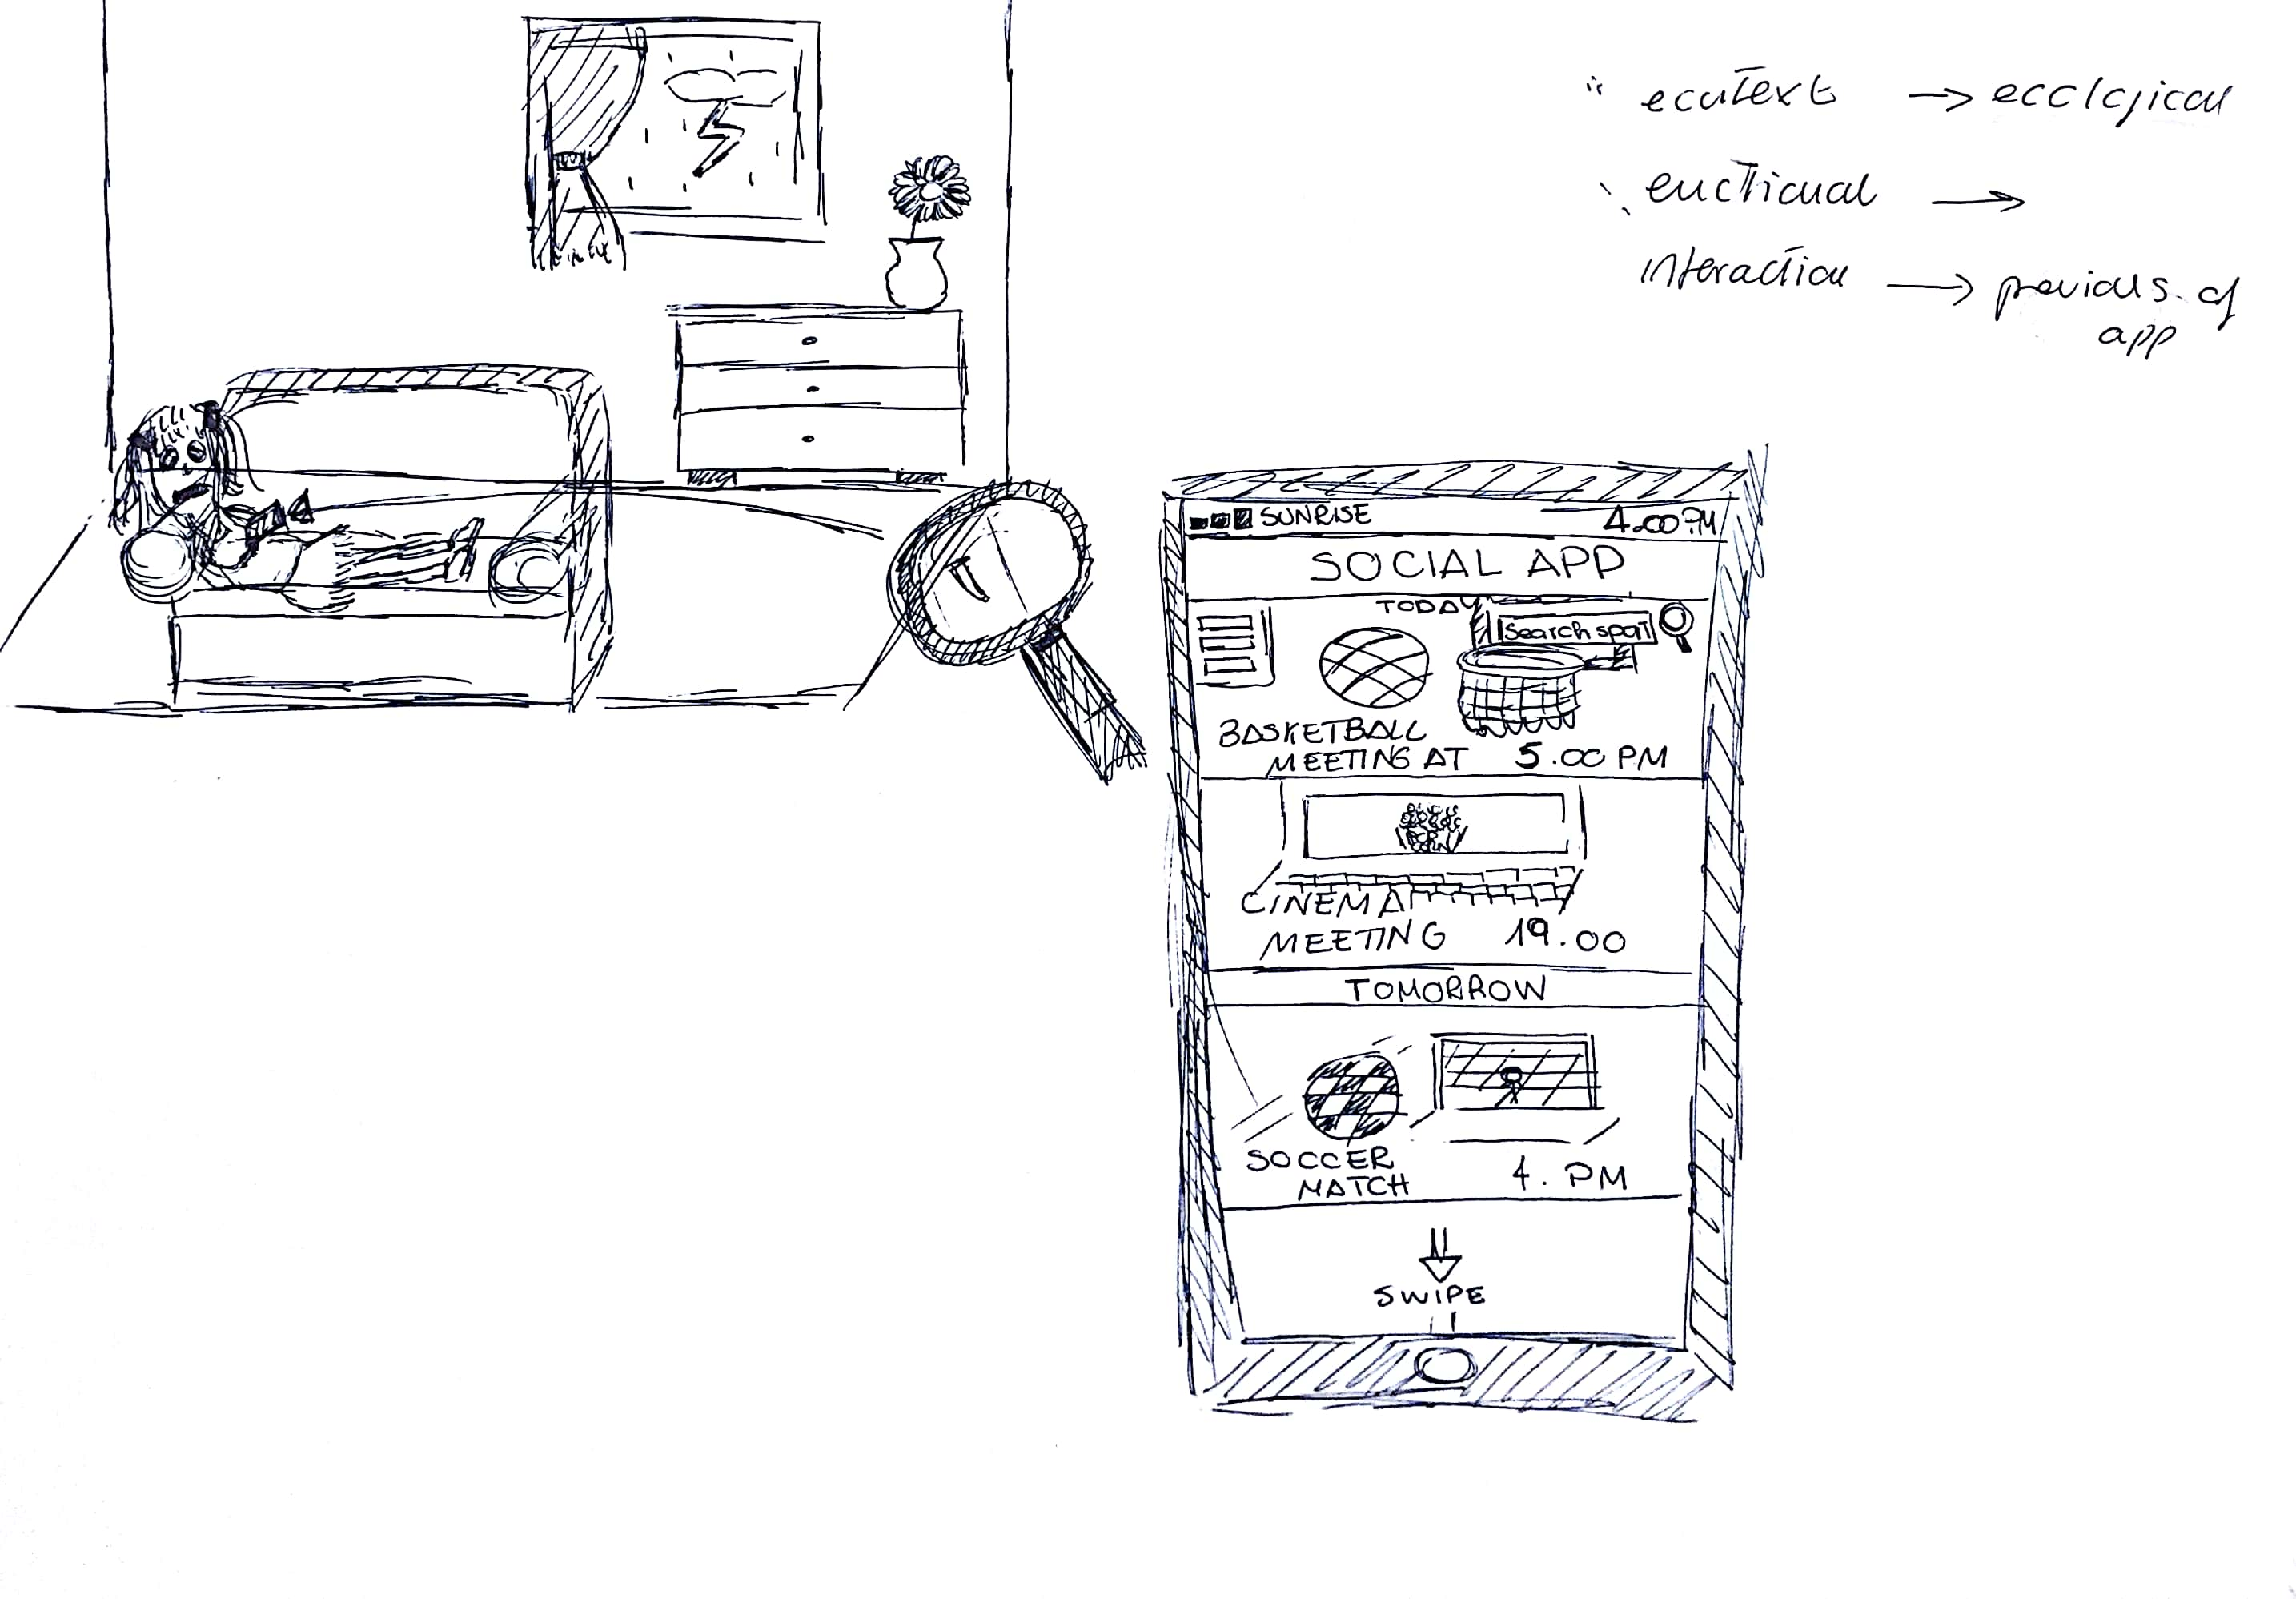
\includegraphics[scale=0.29]{Ecological.jpg}
	\end{figure}
	\\
	Of note is that all of the sketches above also contain some minor storyboard elements. For example, the interaction visualisation briefly touches on our concept of the process that the user would have to go through in order to create an event.
	\newpage
	\section*{\huge Storyboard}
	We have produced two drawn app use scenarios. Note that they are read from left to right, top to bottom.\\
	The first storyboard depicts the in-field use of the app. Those feeling bored or lonely can quickly create an open event. Their friends/classmates can be notified through notifications, while others can also see the event in open search or in app notifications. This leads to the event taking place and children making new friends. The other story board is similar, depicting how impactfull real-time search is. Those with no current activity can quickly look up nearby open events, allowing children to connect with one another. What is not shown in the images directly is a communication step that occurs between those who create and those who wish to join the event. Those interested can confirm their attendance at the push of an on-screen prompt, or by contacting the event creator.
	\newpage
	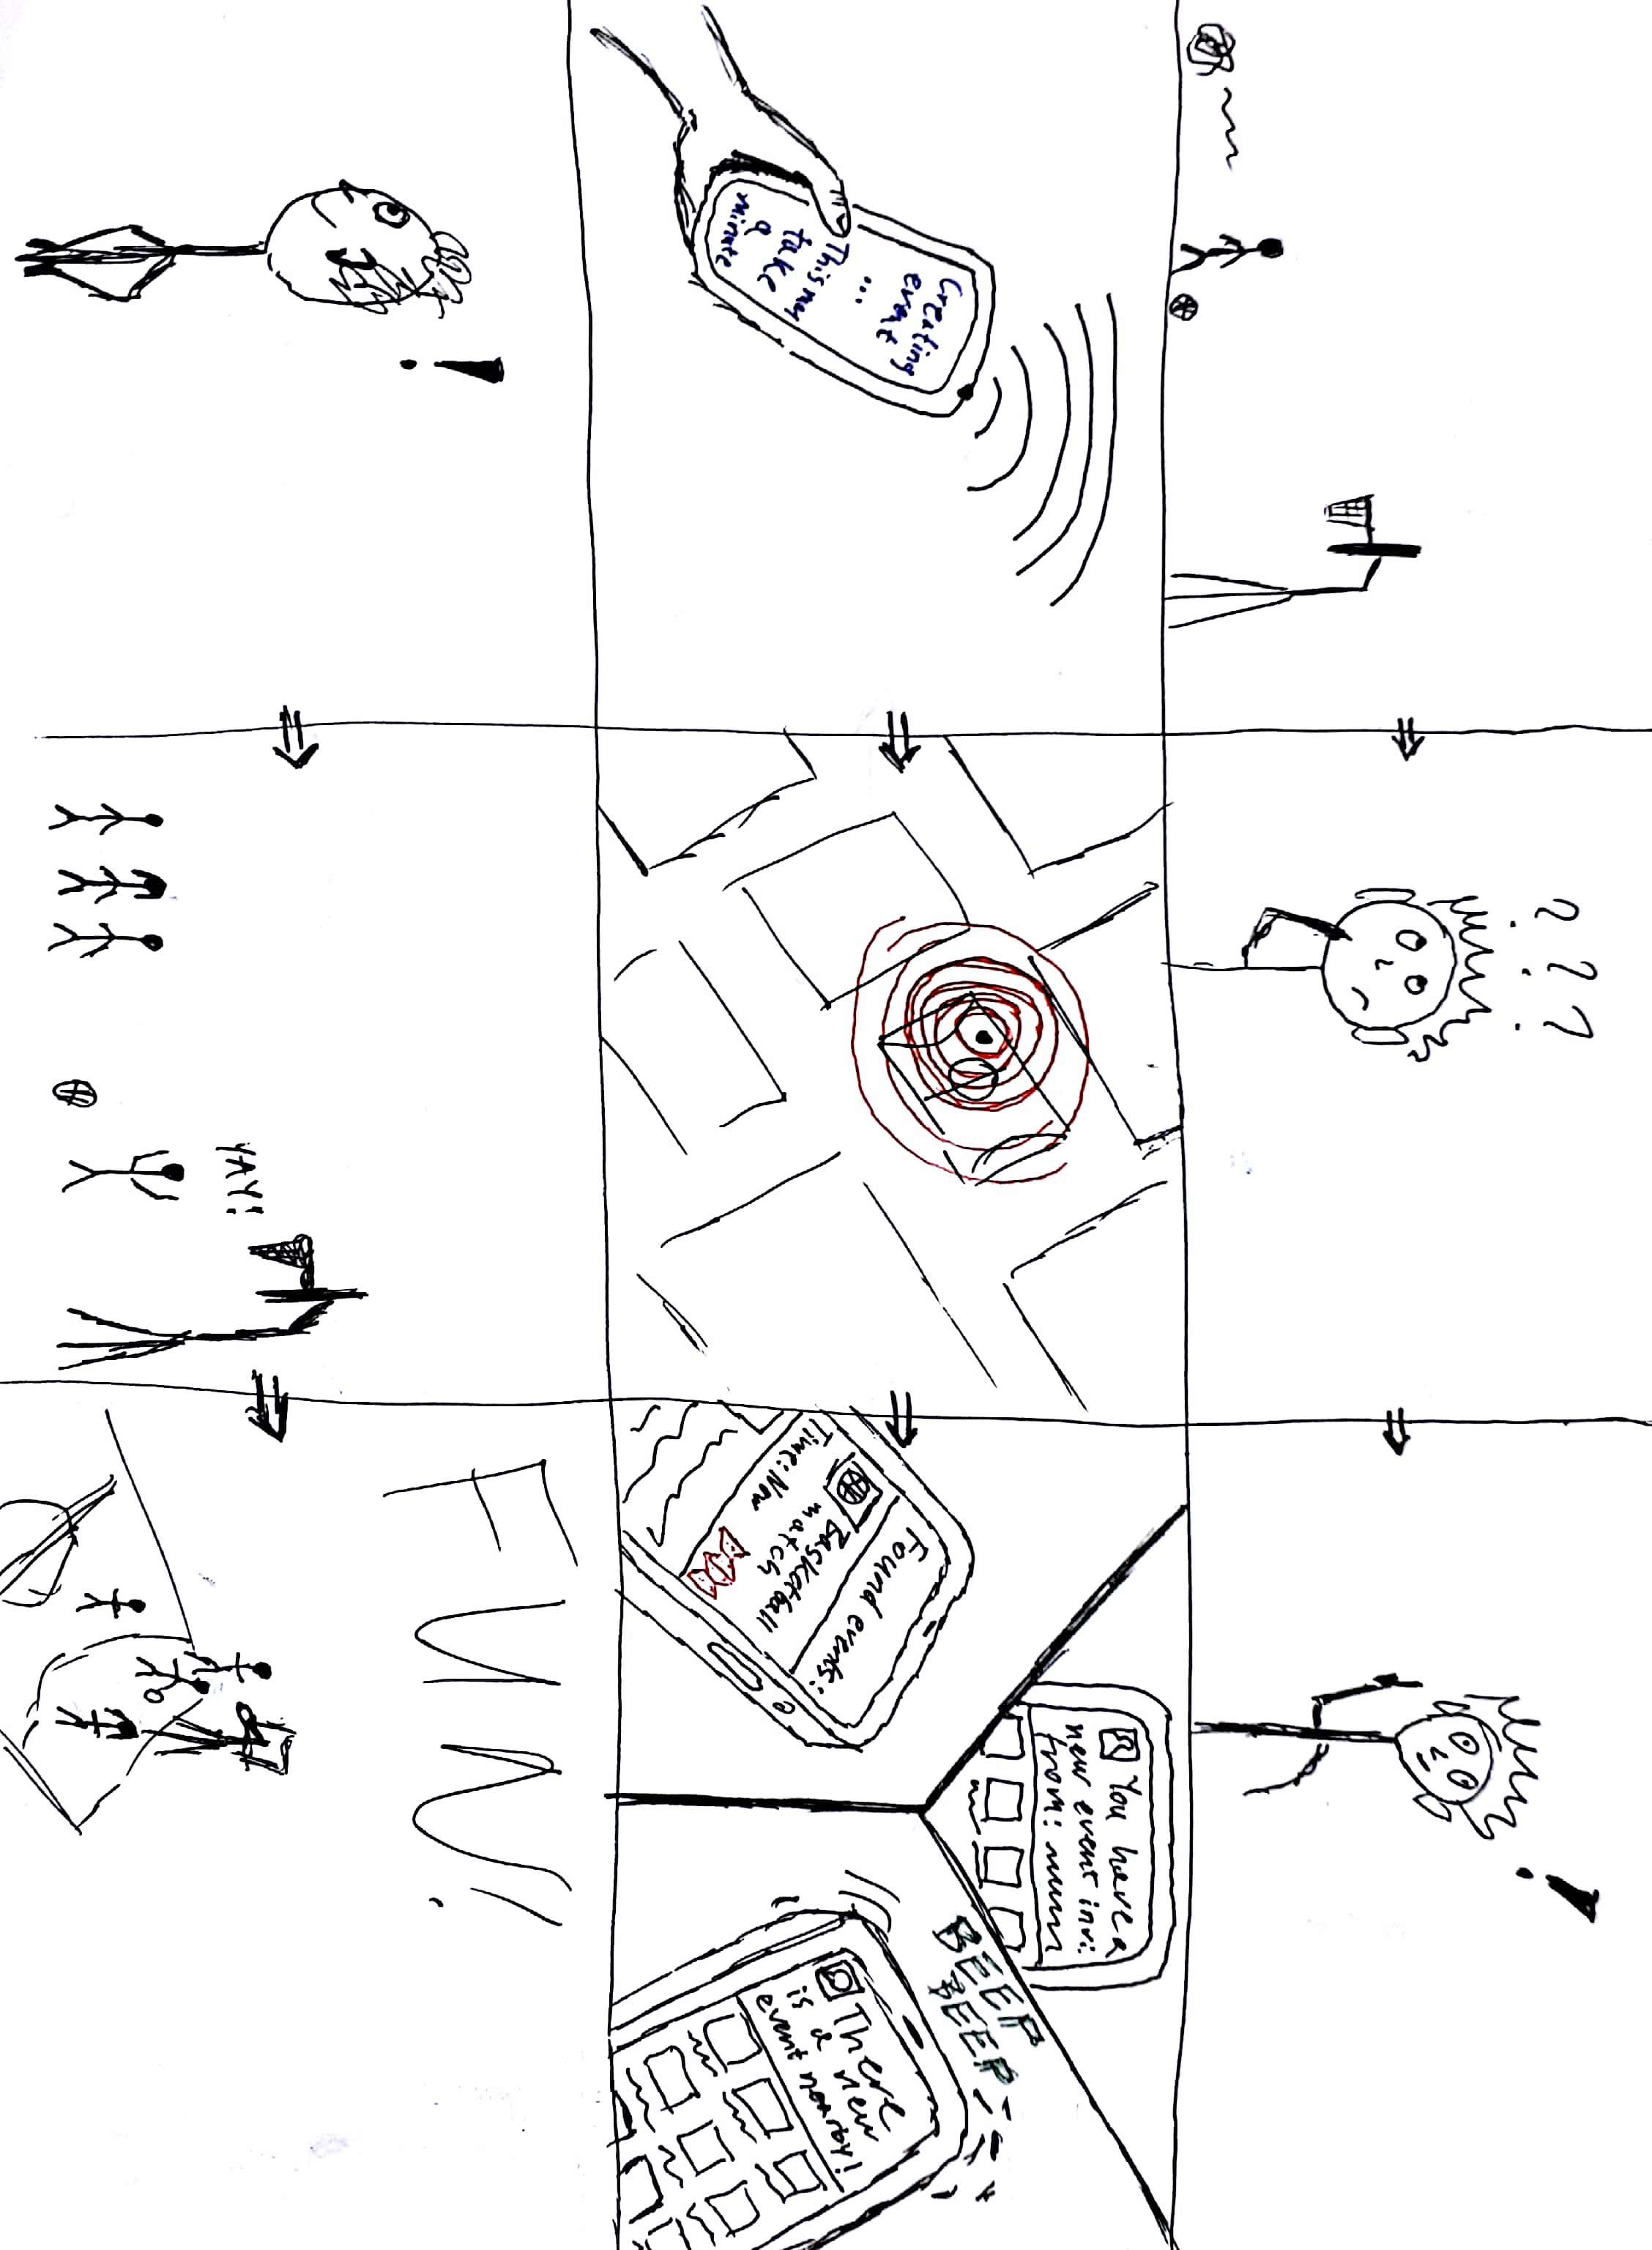
\includegraphics[width=\linewidth]{Story1.jpg}\break
	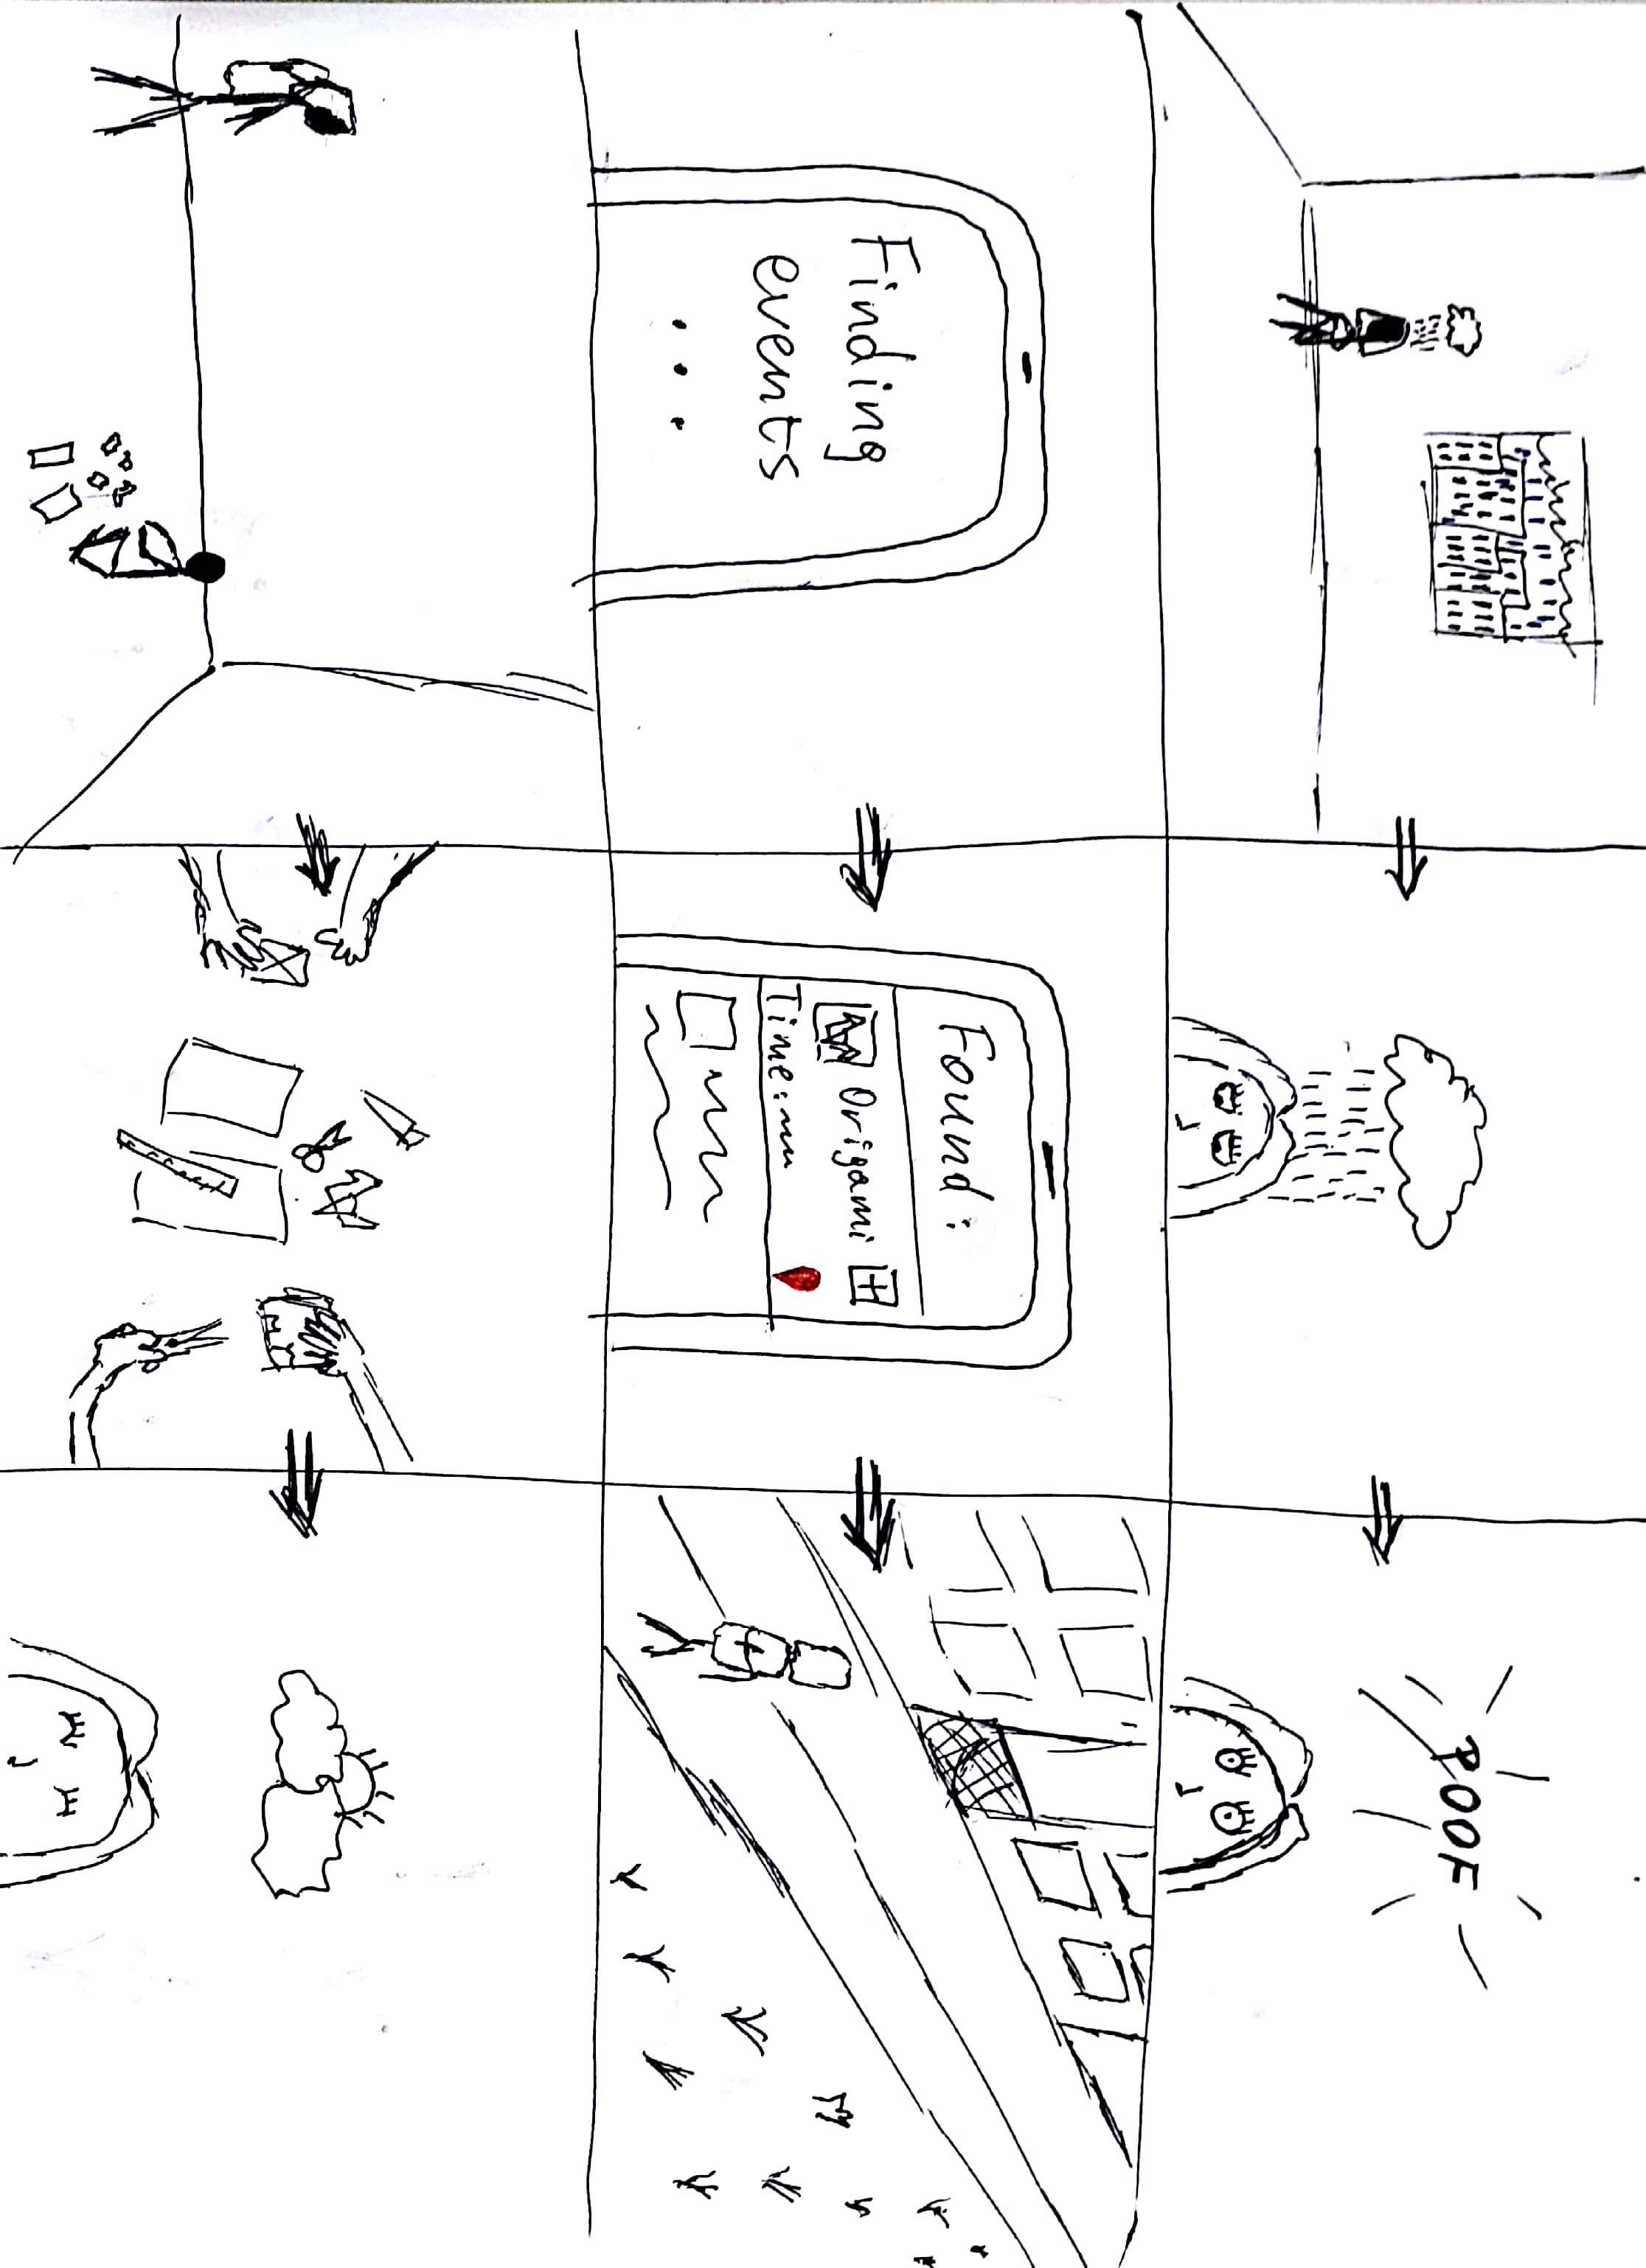
\includegraphics[width=\linewidth]{Story2.jpg}\break
	\end {document}
